\documentclass{article}
\usepackage[utf8]{inputenc}
\usepackage[czech]{babel}

\title{IVS - profiling}
\author{Lidé u výtahu}
\date{April 2020}

\usepackage{natbib}
\usepackage{graphicx}

\begin{document}

\maketitle

\tableofcontents

\section{Úvod}
Pro výpočet výběrové směrodatné odchylky naše skupina zvolila vývoj Konzolové aplikace s názvem SampleStandardDeviation.exe. Tato aplikace používá třídu IVSMath s matematickými operacemi. Ze standardního vstupu načte libovolný počet čísel a na standardní výstup vypíše výběrovou směrodatnou odchylku.

\section{Profiling}
Ve Visual Studiu 2019 jsme naši aplikaci profilovali pomocí Performance profileru, který jako výstup vytváří soubor s příponou .diagsession. Tento soubor obsahuje veškerá data zjištěná při profilování a dá se otevřít přímo ve Visual Studiu. 

Mimo jiné obsahuje tabulku funkcí s jednotkami CPU, které daná funkce spotřebovala za běhu aplikace. Zobrazuje funkce, které spotřebují alespoň jednu jednotku CPU, ostatní nezahrnuje. To stejné platí pro zobrazení náročnosti jednotlivých řádků. Na obrázku 1 je vidět příklad výstupu profileru pro vstup s 1000 čísel. Zobrazuje řádky, které zabírají v průběhu programu nejvíce CPU.

\section{Závěr}
Tato metoda profilování přinesla jasnou představu o tom, které řádky kódu jsou prováděné nejčastěji a zaberou nejvíce času na CPU. 
Při případné optimalizaci bychom se měli soustředit právě na tyto klíčové oblasti.

\begin{figure}[h]
\begin{center}
\centering
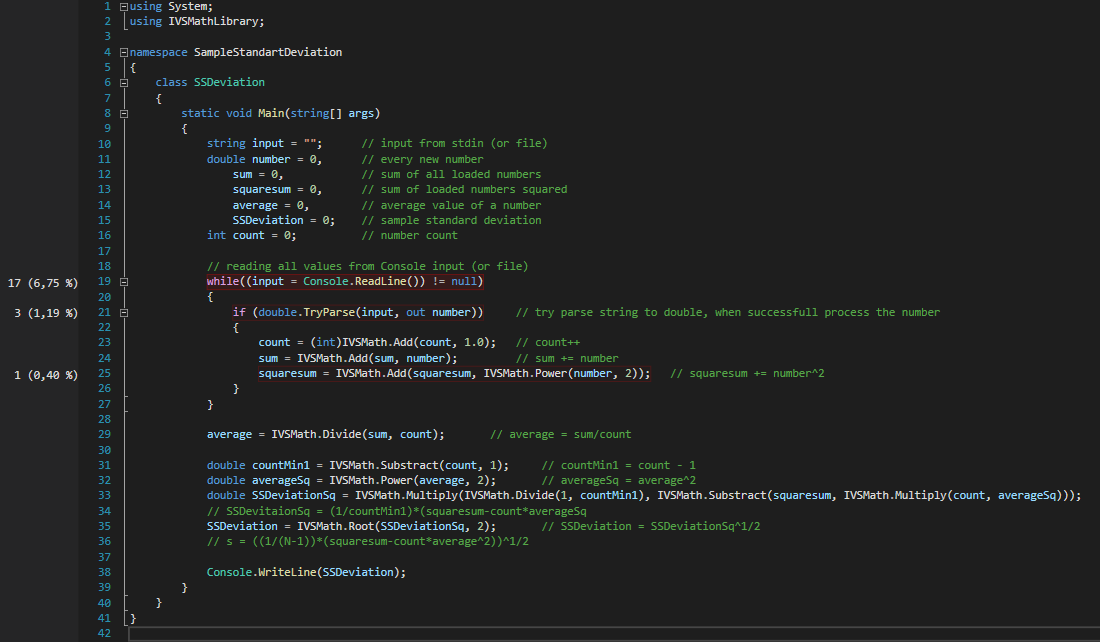
\includegraphics[scale=0.46,valign=t]{vystup-data1000}
\caption{Výstup profileru}
\label{fig:universe}
\end{center}
\end{figure}

\section{Přílohy}
\begin{tabular}[pos]{ | c | c |}
\hline
Název souboru & Popis \\
\hline
vystup-data10.diagsession & výstup profilování s 10 vstupy \\
vystup-data10.png & screenshot využití kódu s 10 vstupy \\
\hline
vystup-data100.diagsession & výstup profilování se 100 vstupy \\
vystup-data10.png & screenshot využití kódu se 100 vstupy \\
\hline
vystup-data1000.diagsession & výstup profilování s 1000 vstupů \\
vystup-data10.png & screenshot využití kódu s 1000 vstupů \\
\hline
\end{tabular}

\end{document}
